\section{Ergebnisse}
Die in der Fallstudie betrachteten Beispiele zeigen, dass es verschiedene Möglichkeiten für Individuen gibt, ihre persönlichen Daten zu monetarisieren. Während sich die Plattformen in einigen Funktionen unterscheiden, funktionieren sie im Grunde nach demselben Prinzip. Als erstes werden Daten erhoben oder eingebunden, damit sie im zweiten Schritt aufbereitet und weiterverarbeitet werden können. Individuen erhalten hierfür im dritten Schritt einen Gegenwert. Im folgenden Abschnitt werden die Dienste anhand dieser Wertschöpfungskette in drei wesentlichen Punkten verglichen: der Art der Datenerhebung, der Kontrolle und Transparenz über erhobene Daten und abschließend dem Gegenwert, den Individuen für das Teilen ihrer persönlichen Daten erhalten.

\subsection{Datenerhebung}
Datenerhebung meint die Art, wie Dienste an persönliche Daten gelangen bzw. wie Individuen ihre Daten aktiv einbringen können. \newline

\noindent Die beiden Dienste BitsAboutMe und Invisibly unterscheiden sich in diesem Punkt kaum. Auf beiden Plattformen können Benutzer verschiedene Datenquellen, wie beispielsweise Konten aus sozielen Medien oder Bankkonten, einbinden. Das Datum-Projekt verfolgt auch den Ansatz, dass Benutzer externe Dienste als Datenquellen verlinken und so ihre persönlichen Daten teilen. Zum aktuellen Zeitpunkt ist jedoch keine Liste mit möglichen Quellen bekannt. Bei dieser Art der Datenerhebung agieren Individuen lediglich insoweit aktiv, indem sie andere Plattformen verlinken, auf denen bereits personenbezogenen Daten aggregiert worden. \newline

\noindent Auf der anderen Seite steht die Datenerhebung durch das aktive Einbringen neuer persönlicher Daten. Bei BitsAboutMe und Invisibly haben Benutzer die Möglichkeit, eigene Aussagen zur Vervollständigung des Profils zu machen. Personen können Daten aus erster Hand aktiv einbringen, indem sie den eigenen Steckbrief ausfüllen oder mit dem persönlichen Feed interagieren. BitsAboutMe bietet zudem den Dienst an, Kassenzettel einzuscannen. \newline

\noindent Bei den beiden Bonusprogrammen von Payback und Kaufland können Individuen selbstständig Ihre Daten preisgeben, dabei gibt es Basisdaten die von den Individuen eingegeben werden müssen und freiwillige Angaben. Erst mit der Angabe der Daten können diese am Bonusprogramm teilnehmen bzw die gesammelten Treuepunkte der Bonusprogramme in Prämien eintauschen.

\subsection{Kontrolle und Transparenz}
Kontrolle bezeichnet den Umfang der aktiven Teilnahme für Individuen beim Benutzen der Plattformen. Dabei ist es wichtig zu unterscheiden, wie groß die Kontrolle einerseits beim Teilen der Daten und andererseits im Nachhinein beim Entfernen ist. Transparenz meint im Kontext der Datenökonomie, in welchem Umfang Benutzer zu einem bestimmten Zeitpunkt über die Verwendung ihrer persönlichen Daten informiert werden. \newline

\noindent Bei den Diensten BitsAboutMe, Datum und Invisibly gilt, dass Benutzer bei der Datenerhebung im Allgemeinen die volle Kontrolle über ihre persönlichen Daten haben. Auf jeder der drei Plattformen ist es Individuen freigestellt, welche externen Datenquellen sie einbinden möchten und welche nicht -- keine Quelle wird erzwungen. Dabei ist es jedoch wichtig zu erwähnen, dass bei der Registrierung auf allen Plattformen die Angabe von Name und E-Mail-Adresse erforderlich ist. Betrachtet man die detailierte Kontrolle beim Einbinden einzelner Datenquellen, so ist festzustellen, dass Personen keine Entscheidungsgewalt haben. Das bedeutet, Benutzer können plattformseitig zunächst nicht einstellen, welche Datensätze konkret aus einer externen Datenquelle übernommen werden sollen. Dies liegt zum Teil daran, dass es sich an dieser Stelle meist um Rohdaten handelt, die erst später zu aussagekräftigen persönlichen Daten aufbereitet werden. \newline

\noindent Bezüglich der Kontrolle und Transparenz über persönliche Daten, die bereits mit den Plattformen geteilt wurden, unterscheiden sich die Fälle stark. \newline

\noindent BitsAboutMe bietet seinen Benutzern eine umfangreiche Kontrolle über die eigenen Daten an. Personen können nachträglich für jede eingebunde Datenquelle entscheiden, welchen konkreten Datensatz sie teilen bzw. löschen wollen. So lassen sich beispielsweise einzelne Beiträge aus dem Instragram-Feed oder abgespielte Lieder von Spotify entfernen. Zudem lassen sich ganze Datenquellen einfach entfernen, wodurch alte Daten automatisch von der Plattform gelöscht werden. Darüber hinaus werden Benutzer stets transparent über die Verwendung ihrer persönlichen Daten aufgeklärt. Bei jedem Angebot teilt die Plattform mit, sowohl welche Profil- als auch Rohdaten mit Dritten geteilt werden und zu welchem Zweck die Daten verwendet werden. Außerdem werden Individuen darüber informiert, wie die Verarbeitung abläuft. Dies beinhaltet insbesondere die Art der Speicherung -- beispielsweise Auswertung auf Servern des Datenkonsumenten -- und die Dauer des Zugriffs. \newline

\noindent Bei Datum stehen dem Nutzer insgesamt fünf Optionen zur Kontrolle über persönliche Daten zur Verfügung. Mit diesen können Personen einschränken, mit welchen Datenkonsumenten die Daten geteilt werden und ob generell eine Gebühr erforderlich ist. Es ist jedoch nicht ersichtlich, ob diese Einstellungen neben einer ganzen Datenquelle auch auf einzelne Datensätze anwendbar sind. Zudem bleibt die Frage offen, inwiefern Individuen ihre persönlichen Daten aus dem verteilten Speicher entfernen können. Mit jedem Datenzugriff durch Dritte werden Personen in einem Transparenzbericht über die Nutzung ihrer Daten informiert. Dabei ist es wichtig zu erwähnen, dass dieser Bericht erst \textit{nach} der Verwendung erstellt wird und somit bereits ein Verkauf stattgefunden hat. \newline

\noindent Obwohl Invisibly mit viel Kontrolle über die eigenen Daten wirbt, stehen Benutzern in der aktuellen Beta-Phase noch wenige Optionen zur Verfügung. Dabei ist es jedoch wichtig zu erwähnen, dass die Plattform nicht direkt getestet werden konnte und alle Informationen somit auf externen Quellen beruhen. Benutzer können geteilte Datenquellen jederzeit entfernen und dadurch den Zugriff für Invisibly widerrufen. Es bleibt aber die Frage offen, was danach mit den bereits durch Invisibly aggregierten Informationen geschieht: Da die Plattform persönliche Daten zur Erstellung eines detaillierten Profils weiterverarbeitet und keine Rohdaten direkt verkauft, können bereits verarbeitete Informationen nicht ohne Weiteres aus dem Profil entfernt werden. Individuen haben allerdings die Möglichkeit, Invisibly direkt zu kontaktieren und um die Löschung von persönlichen Daten zu bitten. Auf diese Weise können sie ebenfalls einen Download ihrer Daten anfordern, welcher als Transparenzbericht über das eigene Profil dient. \newline

\noindent In Bonusprogrammen haben Individuen keine komplette Kontrolle über Ihre Daten. Es gibt Basisdaten die definitiv eingetragen werden müssen und damit verarbeitet werden. Nur über die freiwilligen Angaben haben die Benutzer die Kontrolle, denn diese müssen nicht preisgegeben werden. Darüber sollten die Individuen sich vor Teilnahme am Bonusprogamm bewusst sein. Weiterhin besteht die Möglichkeit der Einstellung der Datenverarbeitung zu Marketingzwecken, das bedeutet der Benutzer kann entscheiden, ob er individualiserte Werbung erhalten möchte oder nicht. Ebenfalls ob seine Daten zum Kaufverhalten erhoben werden. In den AGB´s und Datenerhebungen, sowie Datenschutz der Bonusprogramme ist einzusehen welche Daten erhoben werden und an wen diese übermittelt werden. Bei Payback und Kaufland ist die Übermittlung an Dritte weitestgehend ausgeschlossen, die Daten werden nur unter den Vertragspartnern übermittelt. Selbstverständilich können Individuen ihre Benutzerkonten schließen. Hierbei unterscheidet Kaufland die Löschung der Kaufland Card und die Löschung des Benutzerkontos, beides muss seperat gelöscht werden. Bestehen noch Punkte auf der Karte so werden diese mit gelöscht. Hingegen bei Payback erfolgt die Löschung der Daten zwar prinzipiell genau, allerdings werden diese für steuerrechtliche Zwecke dennnoch 10 Jahre lang aufgehoben. Bei beiden Programmen können die Individuen jederzeit ihre Daten anpassen, z. B. bei Umzug mit einer neuen Adresse.

\subsection{Gegenwert für Individuen}
Auch wenn sich die untersuchten Dienste teilweise deutlich in ihren Funktionen unterscheiden, erhalten Benutzer in jedem Fall einen Gegenwert für ihre aktive Teilnahme an der Datenökonomie. \newline

\noindent Bei den meisten Plattformen handelt es sich dabei um einen monetären Gegenwert. Während Individuen bei BitsAboutMe für jede Transaktion direkt Geld auf ihr Benutzerkonto erhalten, sammeln sie bei Invisibly zunächst Punkte, die sie letztendlich auch in Geld umrechnen und auszahlen können. Auf der Datum-Plattform sammeln Benutzer sogenannte DAT-Token, welche auf Kryptowährungs-Börsen verkauft werden können. \newline

\noindent Dem direkten monetären Erlös stehen alternative Gegenwerte gegenüber, welche auf den einzelnen Plattformen stark variieren. Auf BitsAboutMe erhalten Personen ausführliche Informationen zu ihren persönlichen Daten. Hierfür analysiert der Dienst sämtliche Datensätze aus geteilten Datenquellen und liefert Zusammenfassungen, beispielsweise zum Nutzerverhalten nach der Zeit. Informaionen bekommen Individuen auch auf Invisibly als Gegenwert. Bei dieser Plattform handelt es sich dabei um das persönliche Feed, welches Nutzern für sie relevante Beiträge anzeigt -- basierend auf umfangreichen Analysen der persönlichen Daten. \newline

\noindent Mit der Teilnahme an Bonusprogrammen erhalten Individuen ebenfalls einen Gegenwert dieser kann sehr stark variieren. Mit der Kaufland Card erhält der Benutzer z. B. gegenüber normalen Einkäufern ohne Card Artikel reduzierter, statt 99ct für Haribo zu zahlen, zahlen diese dann 69ct. Die Punkte die bei Payback und Kaufland gesammelt werden können in Rabatte oder andere Prämien umgewandelt werden. Bei Cashback Programmen, z. B. shoop, erhält das Individuum statt einer Prämie einen direkten Geldwert auf das Konto zurück. 

\subsection{Bonusprogramme}

Bonusprogramme unterscheiden sich in Cashback und Payback (Treuepunkte). \newline

\noindent Bei Payback werden Treuepunkte gesammelt, die anschließend ab einer gewissen Punkteanzahl in Gutscheine bzw. Voucher eingelöst werden können. Zum Beispiel bei Fluglinien können Personen Flugmeilen sammeln, welche für Freiflüge, Upgrades, Hotelübernachtungen oder Mietwagen eingelöst werden können. Bei Payback bleibt das Geld bzw. die Leistung im Kreislauf des beteiligten Unternehmens. \cite{paycashback_all} \newline

\noindent \textit{``Ob beim Shoppen, Fliegen, Tanken oder Telefonieren: Mit dem Prinzip des Punktesammelns über Payback, Webmiles oder Kundenkarten wie die DeutschlandCard sind Verbraucher in der Offline-Welt seit Jahren bestens vertraut. Mit dem Aufkommen des E-Commerce haben findige Anbieter das Modell der Bonusprogramme erfolgreich in die Onlinewelt übertragen – die Idee des Cashbacks war geboren. Vorreitermärkte sind weltweit die USA und Großbritannien. In Kontinentaleuropa hinkt Cashback hingegen noch hinterher – das Potenzial wird insbesondere im deutschen Markt noch unterschätzt. Doch durch die Verbreitung mobiler Endgeräte steigert sich das Potenzial zusätzlich.'' \cite{Bonus_affiliate}} \newline

\noindent Beim Cashback bekommt der Kunde bares Geld zurück, welches er woanders wieder investieren kann. Einige Cashback Anbieter erhalten eine Provision durch sogenannte Affiliate Links, in dem über das Portal der Verkauf bestätigt wird. \cite{cashback-vergleich} \newline

\noindent Für den Erhalt des Geldes muss der Kunde/ Teilnehmer seine Kontodaten bekanntgeben. \cite{paycashback_all} \newline



\begin{figure}[!ht]
	\centering
	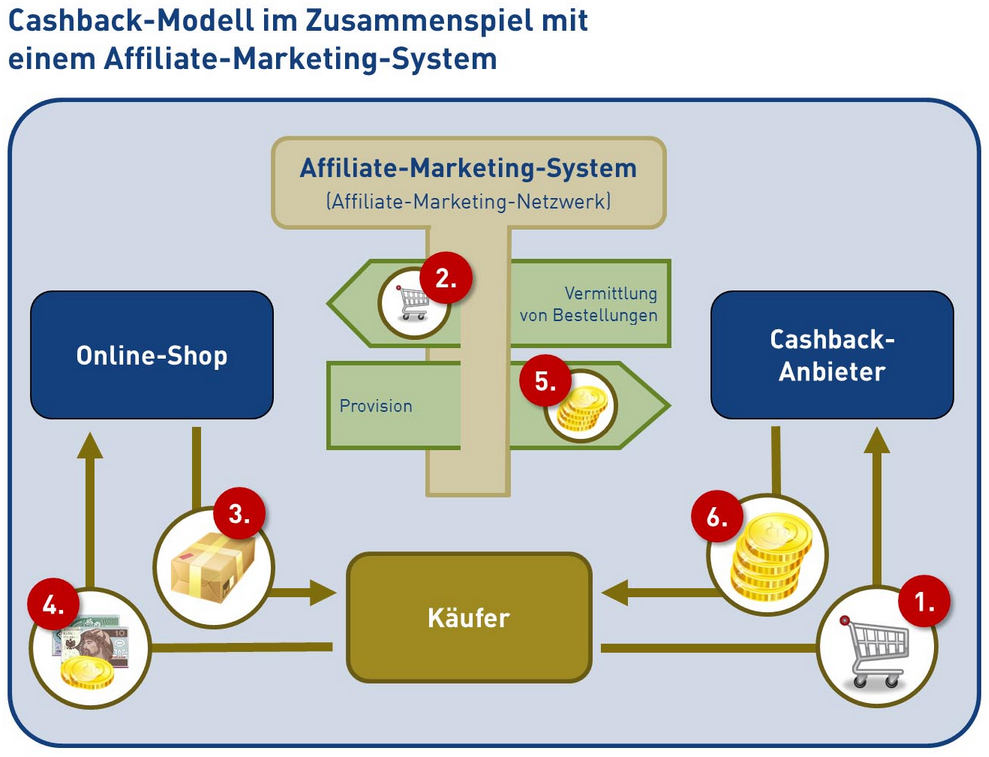
\includegraphics[width=0.8\textwidth]{Cashback-Modell im Zusammenhang mit einem Affiliate-Marketing-System}
	\caption{Cashback-Modell im Zusammenhang mit einem Affiliate-Marketing-System \cite{Bonus_affiliate} }
	\label{fig:Bonus_affiliate}
\end{figure}
\FloatBarrier

\begin{enumerate}
	\item Kunde kauft über ein Cashback-Anbieter in einem Online-Shop ein.
	\item Die Bestellung wird über das Affiliate-Netzwerk an den Online-Shop übermittelt.
	\item Der Online-Shop versendet die Ware an den Käufer.
	\item Der Käufer zahlt an den Online-Shop.
	\item Der Online-Shop zahlt die Provision über das Affiliate-Netzwerk an den Cashback-Anbieter.
	\item Der Cashback-Anbieter zahlt an den Käufer den Einkaufsrabatt (Cashback) \cite{Bonus_affiliate}
\end{enumerate}

\noindent Der wesentliche Unterschied zwischen Cashback und Payback liegt darin, das mit Cashback direkt nach jedem Einlauf Geld erstattet wird, welcher auf das Bankkonto des Kunden gutgeschrieben wird. Zum Beispiel gibt es Aktionen 3 für 2 (1x wird direkt ausgezahlt) im Einzelhandel von Weichspüler oder Schokolade. Dazu muss man in dem Aktionszeitraum die Produkte einkaufen und anschließend den Kassenzettel hochladen. Danach bekommt man das Geld erstattet, welches zuerst vom Kunden ausgegeben wurde. Payback kann erst im Anschluss ab einer gewissen Punktemenge in Prämien oder Gutscheinen eingelöst werden. \cite{TreueCash} \newline

\noindent Es gibt verschiedene Anbieter für Bonusprogramme z.B. für Treuepunkte sei genannt DeutschlandCard, Payback, Webmiles, KauflandCard, DM. Für Cashback-Programme z. B. card4you, Shoop. Weiterhin existieren noch viele weitere Anbieter, in dieser Arbeit wird im Punkt \ref{Payback} auf Payback eingegangen und die KauflandCard.

\subsection {Ziele}
Die Ziele von Bonusprogrammen sind: \newline

\noindent \textbf{Kundenbindung:} \textit{``Bei Payback und Cashback erhalten Kunden für ihren Einkauf Prämien, Gutscheine oder bares Geld zurück. Je regelmäßiger man kauft und je mehr man dabei ausgibt, desto höher fällt üblicher Weise auch der Benefit aus. Bonusprogramme wie Payback oder Cashback spielen daher eine wichtige Rolle bei der Kundenbindung. Ziel der Kundenbindung ist es, aus Laufkundschaft Stammkunden zu machen sowie treue Kunden mit einem besonderen Bonus zu belohnen. Um das zu erreichen, stellen Unternehmen oft Vorteile in Aussicht, die nur für die Teilnehmer des Programms gelten. Das können zum Beispiel Rabatte beim Kauf, eine bevorzugte Behandlung – zum Beispiel eigene Parkplätze – oder eben Prämien für einen getätigten Einkauf sein. Kundenbindung gelingt dann, wenn verschiedene Faktoren zusammenspielen: ein gutes Serviceangebot, bequeme Öffnungszeiten und attraktive Zusatzleistungen.'' \cite{paycashback_all}} \newline

\noindent \textbf{Kundendaten erheben und auswerten:} \textit{``Zusätzlich zur Kundenbindung helfen Loyalty-Systeme wie Bonusprogramme dabei, präzise Daten über Kunden und deren Einkaufsverhalten zu sammeln und zu analysieren. Inwieweit und in welchem Ausmaß diese Daten gesammelt werden, variiert dabei von System zu System. Bei der Teilnahme an einem Kundenbindungsprogramm wie Payback oder Cashback willigen Kunden ein, dass ihr komplettes Einkaufsverhalten erfasst und ausgewertet wird. Welche Informationen sie zur Teilnahme angeben müssen, ist von Programm zu Programm ebenfalls unterschiedlich. Da Kunden bei Cashback Geld überwiesen bekommen, ist in jedem Fall die Angabe der Kontoverbindung erforderlich.'' \cite{paycashback_all}} \newline

\noindent \textbf{Kundenbindungsprogramme steigern den Umsatz durch neue Kunden:} \textit{``Payback und Cashback haben gemein, dass sie die Kundenbindung erhöhen. Dank des bestehenden Mitglieder-Pools der Shopping-Community können teilnehmende Unternehmen zudem neue Kunden gewinnen und in Folge dessen ihren Umsatz erhöhen. Dadurch steigt auch die Zahl der Stammkunden, die regelmäßig einkaufen. Mitglieder eines Loyalty-Programms beziehungsweise Kundenbindungsprogramms sind loyal gegenüber ihren Einkaufsstätten und liefern so einen deutlich höheren Durchschnittsumsatz als reguläre Kunden. Hinzu kommt, dass die Teilnehmer eines Bonusprogramms in der Regel eher bei einem Partnerunternehmen als bei einem Unternehmen außerhalb der jeweiligen Shopping-Community einkaufen. Ein weiterer Vorteil ist, dass Unternehmen direkt mit ihren Kunden kommunizieren können, zum Beispiel durch personalisierte Newsletter.'' \cite{paycashback_all}} \newline